\documentclass{article}
\usepackage{graphicx}
\usepackage{amsmath}

\title{Our First Document}
\author{Jarosław Karczmarczyk}
\date{}

\begin{document}
\pagestyle{empty}
\begin{center} \section*{The Boat} \end{center}


\noindent Let’s imagine that you’re designing the part of boat navigation system. The boat is moving from one point to next point along the line. It is possible to change course only at the end of line. The course is changing by minimal possible angle. It is expected to determine whether the boat is turned right. The boat is turned right always when the sum of angles is greater than zero. Assume that whenever the boat is turning right then sign of angle is positive and negative when turning left.
\begin{figure}[htpb]
\begin{center}
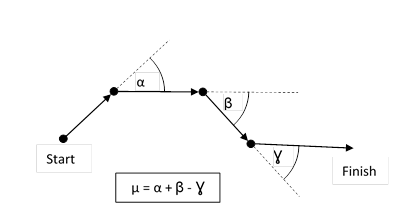
\includegraphics{boat_path.png}
\caption{How to determine sum of angles}
\label{boat_path}
\end{center}
\end{figure}


\noindent In the Figure~\ref{boat_path}, sum of angles is represented by \(\mu\) and when it is greater than zero then boat is turned right. 

\subsection*{Input}
The input is composed of two lines. First line contains one integer number \(0 \leq n \leq 1000000\) which is always even number. This is the number of numbers in next line. 
In the second line there is a sequence of numbers which should be considered as pairs describing points. In every pair first number \(0 \leq x \leq 1 000 000\) is X coordinate and second number \(0 \leq y \leq 1 000 000\) is Y coordinate. Sequence of points is path of sailing boat. 

\subsection*{Output}
Output contains always only one line with “True” or “False” word. 
If it is possible to determine whether the boat is turned right and if it is turned right, then in the output program should put “True” word. In every other situation it is expected to put “False” word in the output.


\end{document}